%%%%%%%%%%%%%%%%%%%%%%%%%%%%%%%%%%%%%%%%%
% Article EcoFoG
% Version 2.1 (23/10/2017)
%
% adapté de :
% Stylish Article
% LaTeX Template
% Version 1.0 (31/1/13)
%
% This template has been downloaded from:
% http://www.LaTeXTemplates.com
%
% Original author:
% Mathias Legrand (legrand.mathias@gmail.com)
%
% License:
% CC BY-NC-SA 3.0 (http://creativecommons.org/licenses/by-nc-sa/3.0/)
%
%%%%%%%%%%%%%%%%%%%%%%%%%%%%%%%%%%%%%%%%%


%----------------------------------------------------------------------------------------
%	PACKAGES AND OTHER DOCUMENT CONFIGURATIONS
%----------------------------------------------------------------------------------------

\documentclass[fleqn,10pt]{ArtEcoFoG} % Document font size and equations flushed left

\setcounter{tocdepth}{3} % Show only three levels in the table of contents section: sections, subsections and subsubsections


% Pandoc environments
\usepackage{framed}
\usepackage{fancyvrb}
\providecommand{\tightlist}{%
  \setlength{\itemsep}{0pt}\setlength{\parskip}{0pt}}
\newcommand{\VerbBar}{|}
\newcommand{\VERB}{\Verb[commandchars=\\\{\}]}
\DefineVerbatimEnvironment{Highlighting}{Verbatim}{commandchars=\\\{\}, fontsize=\scriptsize} % Code R
\definecolor{shadecolor}{RGB}{248,248,248}
\newenvironment{Shaded}{\begin{snugshade}}{\end{snugshade}}
\newcommand{\KeywordTok}[1]{\textcolor[rgb]{0.13,0.29,0.53}{\textbf{{#1}}}}
\newcommand{\DataTypeTok}[1]{\textcolor[rgb]{0.13,0.29,0.53}{{#1}}}
\newcommand{\DecValTok}[1]{\textcolor[rgb]{0.00,0.00,0.81}{{#1}}}
\newcommand{\BaseNTok}[1]{\textcolor[rgb]{0.00,0.00,0.81}{{#1}}}
\newcommand{\FloatTok}[1]{\textcolor[rgb]{0.00,0.00,0.81}{{#1}}}
\newcommand{\ConstantTok}[1]{\textcolor[rgb]{0.00,0.00,0.00}{{#1}}}
\newcommand{\CharTok}[1]{\textcolor[rgb]{0.31,0.60,0.02}{{#1}}}
\newcommand{\SpecialCharTok}[1]{\textcolor[rgb]{0.00,0.00,0.00}{{#1}}}
\newcommand{\StringTok}[1]{\textcolor[rgb]{0.31,0.60,0.02}{{#1}}}
\newcommand{\VerbatimStringTok}[1]{\textcolor[rgb]{0.31,0.60,0.02}{{#1}}}
\newcommand{\SpecialStringTok}[1]{\textcolor[rgb]{0.31,0.60,0.02}{{#1}}}
\newcommand{\ImportTok}[1]{{#1}}
\newcommand{\CommentTok}[1]{\textcolor[rgb]{0.56,0.35,0.01}{\textit{{#1}}}}
\newcommand{\DocumentationTok}[1]{\textcolor[rgb]{0.56,0.35,0.01}{\textbf{\textit{{#1}}}}}
\newcommand{\AnnotationTok}[1]{\textcolor[rgb]{0.56,0.35,0.01}{\textbf{\textit{{#1}}}}}
\newcommand{\CommentVarTok}[1]{\textcolor[rgb]{0.56,0.35,0.01}{\textbf{\textit{{#1}}}}}
\newcommand{\OtherTok}[1]{\textcolor[rgb]{0.56,0.35,0.01}{{#1}}}
\newcommand{\FunctionTok}[1]{\textcolor[rgb]{0.00,0.00,0.00}{{#1}}}
\newcommand{\VariableTok}[1]{\textcolor[rgb]{0.00,0.00,0.00}{{#1}}}
\newcommand{\ControlFlowTok}[1]{\textcolor[rgb]{0.13,0.29,0.53}{\textbf{{#1}}}}
\newcommand{\OperatorTok}[1]{\textcolor[rgb]{0.81,0.36,0.00}{\textbf{{#1}}}}
\newcommand{\BuiltInTok}[1]{{#1}}
\newcommand{\ExtensionTok}[1]{{#1}}
\newcommand{\PreprocessorTok}[1]{\textcolor[rgb]{0.56,0.35,0.01}{\textit{{#1}}}}
\newcommand{\AttributeTok}[1]{\textcolor[rgb]{0.77,0.63,0.00}{{#1}}}
\newcommand{\RegionMarkerTok}[1]{{#1}}
\newcommand{\InformationTok}[1]{\textcolor[rgb]{0.56,0.35,0.01}{\textbf{\textit{{#1}}}}}
\newcommand{\WarningTok}[1]{\textcolor[rgb]{0.56,0.35,0.01}{\textbf{\textit{{#1}}}}}
\newcommand{\AlertTok}[1]{\textcolor[rgb]{0.94,0.16,0.16}{{#1}}}
\newcommand{\ErrorTok}[1]{\textcolor[rgb]{0.64,0.00,0.00}{\textbf{{#1}}}}
\newcommand{\NormalTok}[1]{{#1}}
\usepackage{longtable,booktabs}
\usepackage{caption}
% These lines are needed to make table captions work with longtable:
\makeatletter
\def\fnum@table{\tablename~\thetable}
\makeatother
% longtable 2 columns
% https://tex.stackexchange.com/questions/161431/how-to-solve-longtable-is-not-in-1-column-mode-error
\makeatletter
\let\oldlt\longtable
\let\endoldlt\endlongtable
\def\longtable{\@ifnextchar[\longtable@i \longtable@ii}
\def\longtable@i[#1]{\begin{figure}[t]
\onecolumn
\begin{minipage}{0.5\textwidth}\scriptsize
\oldlt[#1]
}
\def\longtable@ii{\begin{figure}[t]
\onecolumn
\begin{minipage}{0.5\textwidth}\scriptsize
\oldlt
}
\def\endlongtable{\endoldlt
\end{minipage}
\twocolumn
\end{figure}}
\makeatother

\usepackage{graphicx,grffile}
\makeatletter
\def\maxwidth{\ifdim\Gin@nat@width>\linewidth\linewidth\else\Gin@nat@width\fi}
\def\maxheight{\ifdim\Gin@nat@height>\textheight0.8\textheight\else\Gin@nat@height\fi}
\makeatother
% Scale images if necessary, so that they will not overflow the page
% margins by default, and it is still possible to overwrite the defaults
% using explicit options in \includegraphics[width, height, ...]{}
\setkeys{Gin}{width=\maxwidth,height=\maxheight,keepaspectratio}

% User-adder preamble
\usepackage{textcomp} \DeclareUnicodeCharacter{B0}{\textdegree}
\usepackage{tabu}
\renewenvironment{table}{\begin{table*}}{\end{table*}\ignorespacesafterend}
\hyphenation{bio-di-ver-si-ty sap-lings}

%----------------------------------------------------------------------------------------
%	ARTICLE INFORMATION
%----------------------------------------------------------------------------------------

\JournalInfo{Hal 00679993} % Journal information
\Archive{DOI xxxx} % Additional notes (e.g. copyright, DOI, review/research article)

\PaperTitle{30 Years of Recruitment in Tropical Forest After Selective Logging} % Article title

\Authors{
Ariane MIRABEL\textsuperscript{1*}\\ Eric MARCON\textsuperscript{1}\\ Bruno HERAULT\textsuperscript{2}
} % Authors
\affiliation{
\textsuperscript{1}UMR EcoFoG, AgroParistech, CNRS, Cirad, INRA, Université des Antilles,
Université de Guyane.\\ \hspace{1em} Campus Agronomique, 97310 Kourou, France.\\\textsuperscript{2}INPHB (Institut National Ploytechnique Félix Houphoüet Boigny)\\ \hspace{1em} Yamoussoukro, Ivory Coast
}
\affiliation{*\textbf{Contact}: ariane.mirabel@ecofog.gf, http://www.ecofog.gf/spip.php?article47} % Corresponding author

\Keywords{mot-clés, séparés par des virgules} % Keywords - if you don't want any simply remove all the text between the curly brackets
\newcommand{\keywordname}{Mots-clés} % Defines the keywords heading name

%----------------------------------------------------------------------------------------
%	ABSTRACT
%----------------------------------------------------------------------------------------

\Abstract{
Résumé de l'article.
}

%----------------------------------------------------------------------------------------

\begin{document}

\selectlanguage{english}

\flushbottom % Makes all text pages the same height

\maketitle % Print the title and abstract box

\tableofcontents % Print the contents section

\thispagestyle{empty} % Removes page numbering from the first page

%----------------------------------------------------------------------------------------
%	ARTICLE CONTENTS
%----------------------------------------------------------------------------------------


\section{Introduction}\label{introduction}

Determining the response of tropical forests to disturbance is a key to
predict their fate in a global change context. A vast literature has
successfully modeled the response of tropical forest dynamics, carbon
stocks and fluxes to anthropogenic and natural disturbances
\citep{Gourlet-Fleury2000, Putz2012, Martin2015, Piponiot2016}.
Regarding diversity, however, similar attempts have been hindered by
both the huge biological diversity and the scarcity of long-term
monitoring. If the response to disturbance has been identified for
common species assemblages, it usually remained confined to few
commercial and valuable species
\citep{Sebbenn2008, Rozendaal2010, Vinson2015}. Forest dynamics, though,
result from the constantly evolving interactions and feedbacks among
trees and their environment and could therefore only be assessed through
a complete community-scale approach \citep{DeAvila2016}.

Key to understand communities response to disturbance is to identify the
processes shaping the composition and diversity of recruited trees.
Forests dynamics stem from the suit of recruitment process from seed
production, dispersion and germination to seedlings' and saplings'
growth until the adult stage. Recruitment mechanisms result from the
interplay of deterministic environmental processes, like the exclusion
of stress-intolerant species or the limitation of similarity through
resource competition \citep{Ackerly2003, McGill2006}, and stochastic
processes like random dispersal, recruitment and death
\citep{Hubbell2001}. The deterministic processes are inherently linked
to disturbance regime which locally changes ecosystem's biotic and
abiotic conditions and maintains species able of efficient acquisition
of resource but living shortly and poorly resistant to hazards and
diseases \citep{Denslow1980}. They rely on the Intermediate Disturbance
Hypothesis (IDH) that explains the maintenance of tropical forests
biodiversity by the patchy variability of environmental conditions in
space and time \citep{Guitet2018}. Specifically, in tropical wet forests
changes light availability has a central role enhancing the recruitment
of pioneers and light-demanding species after disturbance compared to
mature stands where more competitive shade bearers dominate. Disturbance
then enlarges the ecological range of species in the community
\citep{Molino2001, Bongers2009} and shapes their taxonomic diversity,
vegetative structure, physiology as well as carbon, nutrients, and water
cycles \citep{Anderson-Teixeira2013}. \textgreater{}\textgreater{}(on
parle plus vraiment de IDH maintenant) Empirical tests of the IDH in
tropical rainforests, though, proved hard to succeed and yielded
controversial results \citep{Hubbell1999, Molino2001, Sheil2003}.

During post-disturbance times, the shift from resource-acquisitive to
resource-conservative ecological strategies may be detected in leaves
(leaf thickness, toughness, chlorophyll content and specific area) and
stem (wood specific gravity and bark thickness) and life-history traits
(maximum height at adult stage and class of seed mass)
\citep{Wright2004, Chave2009b, Herault2011}. The relative importance of
recruitment of new individuals and of mortality of distrubance survivors
will shape the new forest and its functioning. Given that disturbance
survivors largely mirror the pre-disturbance forest composition
\citep{Piponiot2018}, predicting the recruitment composition and
diversity trajectories would be a major step towards the prediction of
the future of tropical forest in a changing global environment where
disturbance are expected to become more and more frequent. This would
give insights into the resilience of this hyperdiverse ecosystems,
elucidate the determinism, or not, of tropical forests trajectories,
test the convergence after disturbance of taxonomic and functional
communities towards initial state and also help future adaptative
conservation strategies \citep{Diaz2005, Gardner2007, Schwartz2017}.

In this paper we follow the fate of a recruited tree communities (60121
individuals) over 30 years on a disturbance gradient, with 10 to 60\% of
forest biomass removed. We assessed the taxonomic as well as functional
diversity of recruited trees, using a large functional trait database
covering, the leaf, wood and life-history spectra. We aimed to (i)
assess the role of environmental filtering selecting the recruited trees
according to their competitivity for resource acquisition, (ii) resolve
the convergence of communities and the maintenance of taxonomic
composition in the long term, and (iii) determine the global resilience
of the ecosystem.

\section{Material and Methods}\label{material-and-methods}

\subsection{Study Site}\label{study-site}

The Paracou station is located in a lowland tropical rain forest in
French Guiana (5°18'N and 52°53'W). Climate is tropical wet with mean
annual precipitation averaging 2980 mm.y\textsuperscript{-1} (30-y
period) and a 3-months dry season (\textless{} 100
mm.months\textsuperscript{-1}) from mid-August to mid-November, and a
one-month dry season in March \citep{Wagner2011}. Elevation ranges from
5 to 50 m and mean annual temperature is 26°C. Soils are thin acrisols
over a layer of transformed saprolite with low permeability generating
lateral drainage during heavy rains. The disturbance experiment spread
over a network of twelve 6.25ha plots (Table \ref{tab:Tab1}) that
underwent three disturbance treatments in 1986-1987 \citep{Herault2018}.
Dominant families are Fabaceae, Chrysobalanaceae, Lecythidaceae and
Sapotaceae.

\begin{table}

\caption{\label{tab:Tab1}Intervention table, summary of the disturbance intensity for the 4 plot treatments in Paracou.}
\centering
\begin{tabu} to \linewidth {>{\raggedright}X>{\raggedright}X>{\raggedright}X>{\raggedright}X>{\raggedright}X}
\toprule
Treatment & Timber & Thinning & Fuelwood & \%AGB lost\\
\midrule
Control &  &  &  & 0\\
T1 & DBH $\geq$ 50 cm, commercial species, $\approx$ 10 trees/ha &  &  & $[12\%-33\%]$\\
T2 & DBH $\geq$ 50 cm, commercial species, $\approx$ 10 trees/ha & DBH $\geq$ 40 cm, non-valuable species, $\approx$ 30 trees/ha &  & $[33\%-56\%]$\\
T3 & DBH $\geq$ 50 cm, commercial species, $\approx$ 10 trees/ha & DBH $\geq$ 50 cm, non-valuable species, $\approx$ 15 trees/ha & 40 cm $\leq$ DBH $\leq$ 50 cm, non-valuable species, $\approx$ 15 trees/ha & $[35\%-56\%]$\\
\bottomrule
\end{tabu}
\end{table}

\subsection{Inventories Protocol and Dataset
Collection}\label{inventories-protocol-and-dataset-collection}

All trees above 10 cm DBH were mapped and measured annually since 1984.
During inventories, trees were first identified with a vernacular name
assigned by the field team, and afterward with a scientific name
assigned by a botanist during regular botanical campaigns. Botanical
campaigns have been carried out every 5 to 6 years from 2003 onwards.
This raised methodological issues as vernacular names usually correspond
to different botanical species, resulting in significant taxonomic
uncertainties that were propagated to composition and diversity metrics.
Vernacular names were replaced through multinomial trials
\(M_v\Big(\big[s_1, s_2, …, s_N\big],\big[\alpha_1, \alpha_2,…, \alpha_3\big]\Big)\)
based on the observed association probability
\(\big[\alpha_1, \alpha_2,…, \alpha_3\big]\) between each vernacular
name \emph{v} and the species \(\big[s_1, s_2, …, s_N\big]\) recorded in
the inventory. See appendix 1 and \citet{Aubry-Kientz2013} for the
detailed methodology. To avoid remaining identification caveats, the
simulated botanical inventories were reported at genus level.

Six functional traits, representing leaf economics (leaves thickness,
toughness, total chlorophyll content and specific leaf area, the leaf
area per unit dry mass), wood economics (wood specific gravity and bark
thickness) and life history traits (maximum specific height and seed
mass), come from the BRIDGE project \footnote{http://www.ecofog.gf/Bridge/}
where trait values were measured on nine french guianan forest plots,
including two in Paracou. Missing trait values (10\%) were filled using
multivariate imputation by chained equation (mice). As traits
variability was lower within species and within genus, we accounted for
the phylogenetic signal of the functional traits in restricting thegap
filling processes to samples pertaining to the next higher taxonomic
level (refs MICE). As seed mass information corresponds to a
classification into mass classes, no data filling process was applied so
analysis were performed only considering the 414 botanical species of
the seed mass dataset.

Functional trajectories were estimated with the Rao quadratic entropy
using community weighted means (CWM) \citep{Diaz2007, Garnier2004}. Seed
mass trajectories were reported by the proportion of each class recorded
in the inventories. All composition and diversity metrics are the
average obtained after 50 iterations of taxonomy and trait values
uncertainty propagation.

\subsection{Recruitment trajectories}\label{recruitment-trajectories}

We split the forest community in `survivors, i.e.~trees that survived
the disturbance, and post-disturbance recruited trees. Two recruitment
metrics were examined: on the one hand the ``punctual recruitment'' by
2-year intervals after disturbance, on the other hand all recruited
trees since disturbance, hereafter ``accumulated recruits''. The
taxonomic diversity was assessed through Richness and the Hill number
translation of Shannon and Simpson indices
\citep{Hill1973, chao2015estimating, Marcon2015b}. These three indices
belong to the set of HCDT or generalized entropy, respectively
corresponding to the 0, 1 and 2 order of diversity (\emph{q}), which
grasps the balance between richness and evenness in the community, with
common species weighting more than rare ones when \emph{q} increases.
The similarity between the recruited trees and the pre-disturbance
forest was measured with the turnover metrics detailed in
\citet{Podani2013a}. To determine whether recruitment trajectories
ensued from a pure random process, observed trajectories were compared
to those generated by 50 repetitions of a random null model shuffling
individuals among plots while preserving species abundance and plots'
tree density.

To draw plots trajectories we applied a moving average with a one step
window allowing to mitigate the heterogeneity of inventory protocols
between years.

\section{Results}\label{results}

\subsection{Recruitment Diversity}\label{recruitment-diversity}

\subsubsection{Taxonomic Diversity}\label{taxonomic-diversity}

Punctual recruits' diversity followed a consistent trajectory among
disturbance treatments with first higher richness and lower evenness
than in control plots and then equivalent richness and lower evenness
(Figure (\ref{fig:Fig1}). For recruits accumulated since disturbance,
the richness (order 0) in highly disturbed plots (T3 and some T2) was
higher than in control plots, consistently with the increase of
recruited trees after disturbance, and the evenness (order 2) was lower,
specifically for the most disturbed plots (Appendix I, fig. S1).

\begin{figure*}

{\centering 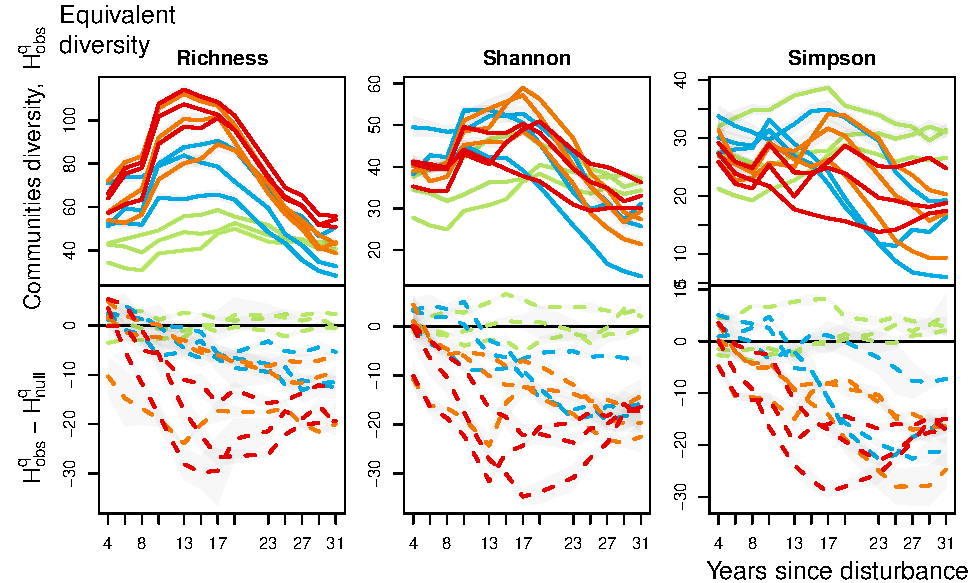
\includegraphics[width=0.8\linewidth]{RecruitmentTrajectories_files/figure-latex/Fig1-1} 

}

\caption{Trajectories of Richness, Shannon and Simpson diversity for 2-years laps punctual  recruitment (upper panels) and divergence to null model (lower panels). Lines colors refer to the perturbation regime: green for control, blue for T1, orange for T2 and red for T3 disturbance treatments. Plain lines correspond to the median observed after uncertainty propagation and are given along with the 95\% confidence interval (grey envelope).}\label{fig:Fig1}
\end{figure*}

Punctual and accumulated recruitment diversity of orders 0, 1 and 2 were
then compared to a null random recruitment model. In control plots the
richness (order 0) and evenness (order 2) of punctual recruits remained
equivalent or higher than for the null random model. For all disturbed
plots in contrast both richness and evenness were lower than these of a
random null model but displayed a significant but unachieved
humped-shaped trajectory for all plots (Figure \ref{fig:Fig1}).
Accumulated recruitment richness and evenness were higher or equivalent
to those of the null model for plots T1 and some plots T2 but lower for
plots T3 and a plot T2 (AppendixI, fig. S1).

\subsubsection{Functional Diversity and
Composition}\label{functional-diversity-and-composition}

The functional diversity (Rao diversity) of punctual recruitment was
measured and compared to a null model of random traits shuffling. In
most distrubed plots (plots T2 and T3) the functional diversity was
deacrinsing and lower to this of control plots until 15 years after
disturbance (Figure \ref{fig:Fig3}). It then increased to values
equivalent or higher to those observed in control plots. For all
disturbed and control plots the observed functional diversity was lower
than for the null model of random traits shuffle, except for two T1
plots.

\begin{figure}

{\centering 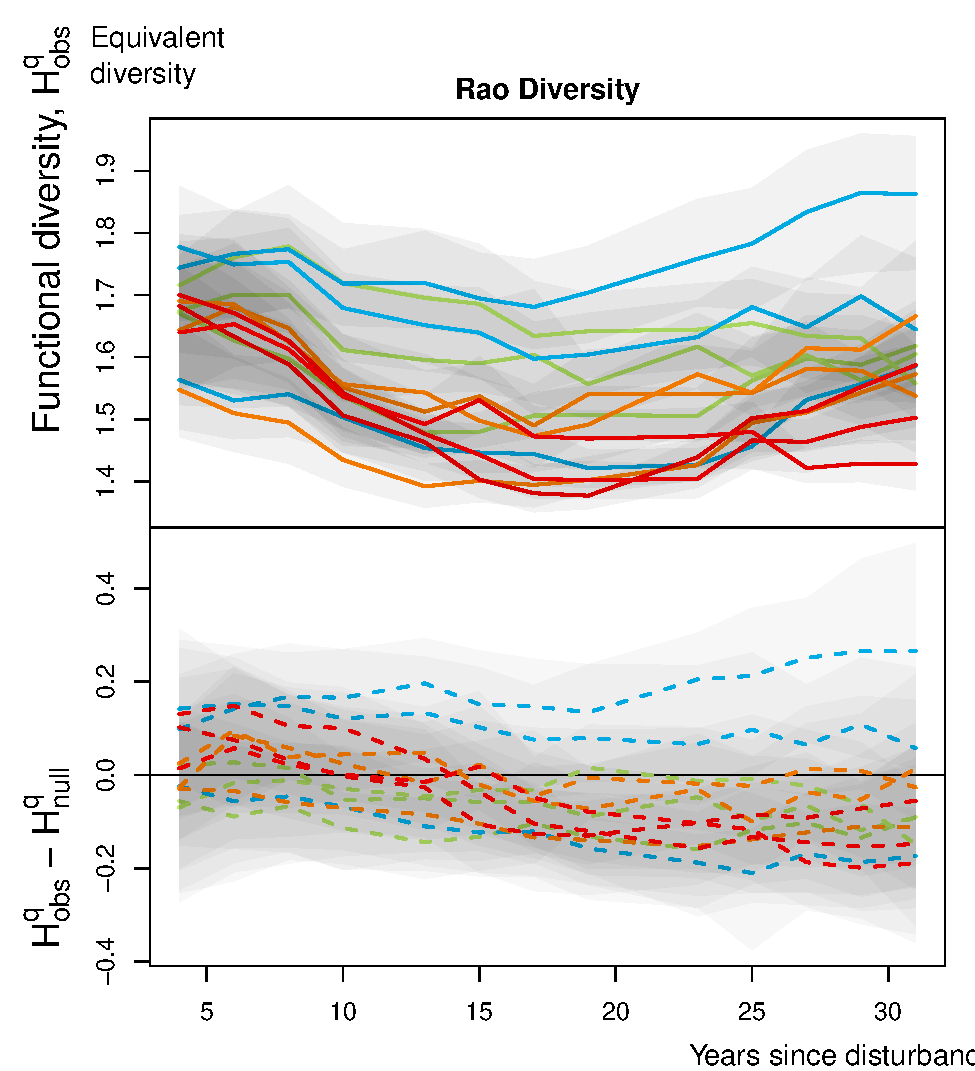
\includegraphics{RecruitmentTrajectories_files/figure-latex/Fig2-1} 

}

\caption{Functional diversity of punctual recruited trees from the considered functional traits and divergence to null model. Values reported correspond to the plot-level median and the 95\% confidence interval obtained after 50 repetition of the taxonomic uncertainty propagation and the functional database gap-filling processes and 50 run of the null model. Lines colors correspond to the logging treatment initially applied (green for control, blue for T1,orange for T2 and red for T3).}\label{fig:Fig2}
\end{figure}

Trajectories of recruited trees in the functional spaces showed the
dominance after disturbance of species displaying large exchange surface
area and light tissues (high SLA, low leaf toughnessand thickness and
low wood specific gravity) (Figure \ref{fig:Fig3}). All traits
trajectories displayed univariate CWM trajectories with leaf toughness,
wood specific gravity and bark thickness decreasing before stabilizing
at low values around 15 after disturbance, except SLA and leaf thickness
that displayed a unimodal trajectory with a maximum reach around 15
years after disturbance.

\begin{figure*}

{\centering 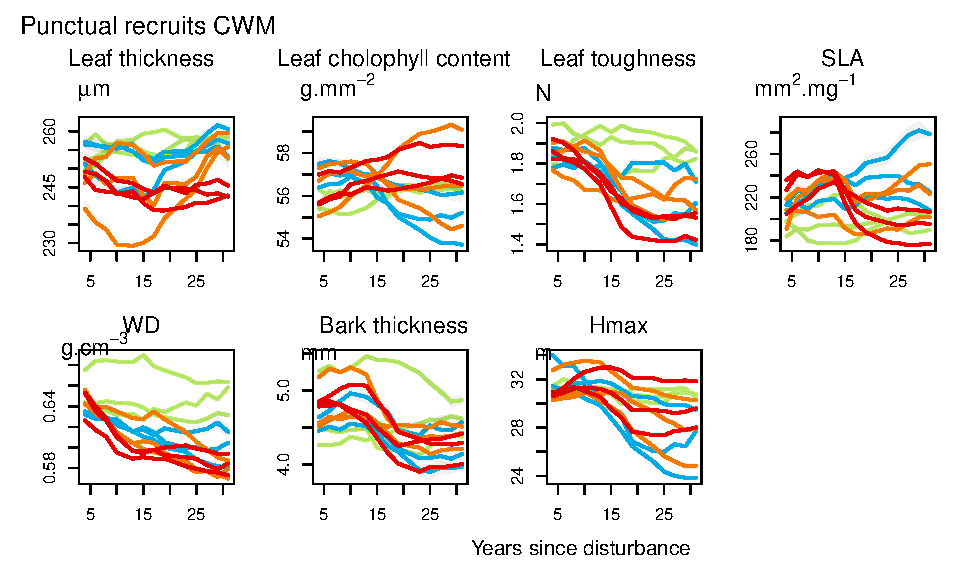
\includegraphics[width=0.8\linewidth]{RecruitmentTrajectories_files/figure-latex/Fig3-1} 

}

\caption{Community weighted means (CWM) of the four disturbance treatment for the four leaf traits, the two stem traits  and the specific Hmax. Values reported correspond to the plot-level median obtained after 50 repetition of the taxonomic uncertainty propagation and the functional database gap-filling processes. Lines colors correspond to the disturbance intensity (green for control, blue for T1,orange for T2 and red for T3).}\label{fig:Fig3}
\end{figure*}

\subsection{Recruitment Turnover}\label{recruitment-turnover}

In control plots species turnover remained highly stable for the 30
sampled years (Figure \ref{fig:Fig4}), reflecting a strong similarity
between the initial plots composition and the punctual recruits. In
disturbed plots, turnover displayed a unimodal response to disturbance,
with maximum reached around 15 years and with a value positively
correlated to the disturbance intensity (\(\rho_{spearman}=0.93\)). The
turnover trajectory returned close to zero for all plots 30 years after
disturbance.

\begin{figure}

{\centering 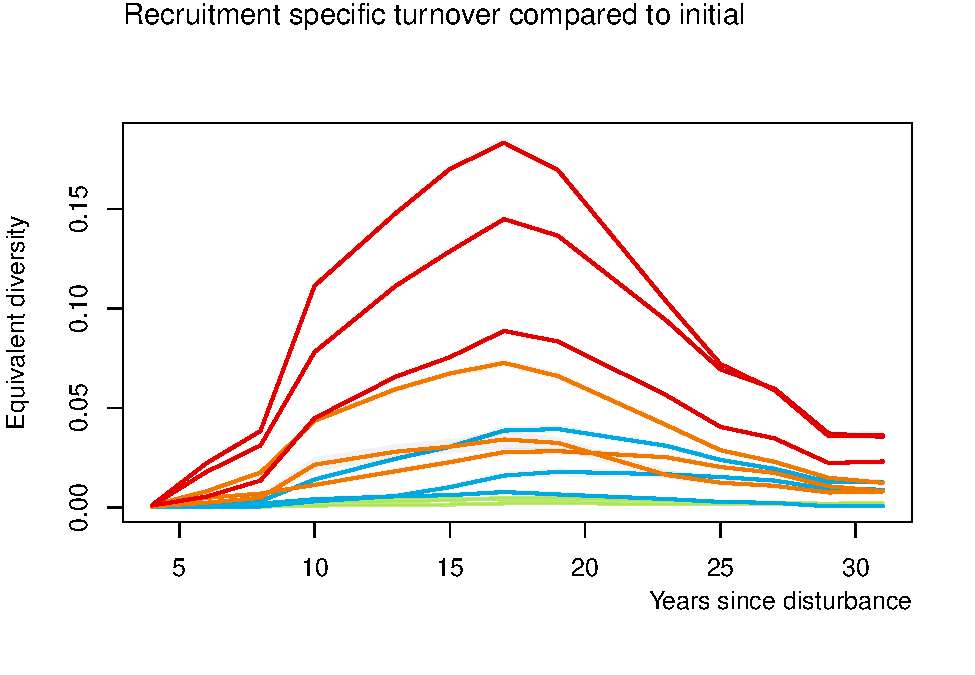
\includegraphics{RecruitmentTrajectories_files/figure-latex/Fig4-1} 

}

\caption{Trajectories over the 30 sampled years of the abundance-based turnover between recruited trees and intial communities before disturbance. Grey envelopes correspond to the 0.025 and 0.975 percentiles of the uncertainty propagation procedue and lines to the median in green for control, blue for T1,orange for T2 and red for T3).}\label{fig:Fig4}
\end{figure}

\section{Discussion}\label{discussion}

From the 30 years monitoring in Paracou forest, we highlighted
contrasting recruitment trajectories determined by the disturbance
intensity. Disturbance increased the number of recruits and hence their
taxonomic richness, but the recruitment was dominated by a pool of
species all the more restricted that disturbance intensity was high.
Recruitment trajectories after disturbance were thus governed by a
gradual balance between deterministic processes, the selection towards
light acquisitive functional strategies and the similarity limitation,
and stochastic processes defining the demography of mature forests. For
the highest disturbance intensity, though, this was preceeded by an
additional phase where the exclusive competition of newly settled hard
pioneers decreased the diversity and changed the composition of
recruited trees. Communities then followed longer-term but similar
trajectories. Pre-disturbance composition, diversity and functioning,
then consistently recovered and initial differences among communities
were maintained. Still, trajectories involved the soil seed bank which
likely altered communities resilience, which questions the consistency
of those trajectories after additional disturbance.

\subsection{On the underlyings of the hump-shaped
trajectories}\label{on-the-underlyings-of-the-hump-shaped-trajectories}

The trajectories of punctual recruitment richness, some key functional
traits (SLA and bark thickness) and the species turn-over exhibited
hump-shaped, unimodal trajectories.

The 10-15 first years of these trajectories seemed driven by the growth
of pre-disturbance saplings benefiting from the environmental changes
and alleviated competition that follow disturbance \citep{Herault2010}.
After low disturbance intensity this translated into a stable functional
diversity of the recruited community, equivalent to this of control
plots that is governed by stochastic recruitment processes. After
intense disturbance, this phase corresponded to sharp increase of SLA
and bark thickness and decrease of wood density weighted means,
revealing prominent recruitment of species with efficient light
acquisition, short-lived tissues and fast growth (Figure \ref{fig:Fig4})
\citep{Wright2004, Chave2009b, Herault2011, Reich2014}. The first
recruitment phase then in addition involved short-lived and competitive
species, \emph{i.e.} hard pionneers, that rapidly dominated the
recruited population and reduced its functional diversity.

Following this first phase, the recruitment progressively incorporated
true recruits, \emph{i.e.} individual trees that had germinated after
disturbance. Disturbance trajectories corresponded to the interplay of
random demographic processes of mature forests that progessively
replaced deterministic processes involving selection and similarity
limitation. The balance between both processes resulted in different
trajectories according to the disturbance intensity.

After low disturbance intensity (T1 plots) the recruitment trajectories
were determined by selective pressures towards light demanding species
that underwent similarity limitation enhancing their functional
diversity. Although the taxonomic composition of the recruitment
resembled the pre-disturbance composition the pool of recruited species
was more restricted and evenly distributed. These restrictions revealed
selective pressures favouring pioneers and light demanding species with
efficient resource acquisition (high SLA and leaf chlorophyll content)
and inexpensive, short-lived tissues (low leaf thickness and thoughness,
small Hmax and low wood density and bark thickness). In parallel the
recruitment's functional diversity increased, equating or exceeding this
of control plots, revealing an overdispersion of functional traits
driven by the limitation of similarity. At this disturbance intensity,
recruitment seemed preserved from the competitive exclusion of hard
pioneers which would have prevented the maintenance of inferior
competitors in the community and would thus have lowered the functional
diversity \citep{Hubbell1999, Sheil2003, Bongers2009}. The low dominance
of hard pioneers might result from recruitment and dispersal limitation
due to the short dispersal distance observed for tropical trees,
specifically in Paracou with the genetic clumping of some pioneers
\citep{Leclerc2015, Scotti2015a}.

The trajectories after intense disturbance, first driven by the
settlement of hard pioneers, progressively matched the same progressive
balance between deterministic and stochastic processes. This translated
by a progressive decrease of recruitment taxonomic turnover and an
increase of functional diversity. Although acquisitive strategies
remained dominant (high leaf chlorophyll content and low wood density
and leaf toughness), the weighted values of other traits stabilized and
the SLA and bark thickness decreased again (then following a unimodal
trajectory with a peak after the first recruitement phase). The 15 years
laps of the unimodal turnover and traits trajectories corresponding to
the first recruitment phase matched the life expectancy of hard pionners
and of their competitive pressure. The recruitment would progressively
shift towards long-lived pionneers which participate to forest recovery
as they might have been part of pre-disturbance communities, but still
hold dominant more acquisitive functional strategies.

\subsection{On the resilience of the recruitment
process}\label{on-the-resilience-of-the-recruitment-process}

Thirty years after disturbance, for all treatments the recruitment
richness and functional diversity had recovered levels equivalent as
those observed short after disturbance and in control plots. In contrast
the species distribution evenness and functional diversity had not
recovered for the most disturbed plots, displaying similar but
unachieved trajectories as those of other plots. Still, the recruitment
processes were restored for all treatments, the recruited species showed
very low turnover compared to initial stands and the difference with
random processes equated those of control plots. This argued for the
high dependence of the composition recovery trajectory on the
pre-disturbance ecosystem characteristics \citep{Anderson2007}. In other
words, initial compositional variation caused tree communities to remain
divergent in taxonomic composition, even though these same tree
communities strongly converged in functional space \citep{Fukami2005}.
This makes these commmunities both functionally and taxonomically
resilient despite the settlment of long lived pioneers which make it a
long term process for high disturbance intensity. Our results extend
previous ones from the Paracou experiment, 10 years \citep{Molino2001}
and 20 years \citep{Baraloto2012a} after disturbance which suggested the
recovery towards pre-disturbance taxonomic and functional composition.

The trajectories of functional traits proved very different among plots
and treatments, sometimes showing opposed tendencies (like for the Leaf
Chlorophyll Content, SLA or Hmax), which suggested that the recovery may
be, more than commonly thought, upon dependence of the pre-disturbance
functional ecosystem signature \citep{Herault2018}. For all traits the
difference with control plots and initial conditions remained marked 30
years after disturbance, although the corresponding functional diversity
had recovered. This supported the role of similarity limitation
increasing maintainting high functional diversity whenever the dominant
strategies.

These concusions however are only valid for a single disturbance event,
give nthat the second recruitment phase involves the seed bank and
therefore triggers a storage effect likely to modify the recruitment
trajectories after an other disturbance event. In this hypothetical
case, the competitive exclusion among dormant life-stage (seeds or even
seedlings) would be harsher and likely bring more radical changes in the
recruitment composition and functional profile.

\section{Conclusion}\label{conclusion}

The long-term study of recruitment diversity trajectories disentangle
the mechanisms ruling recruitment dynamics after disturbance. While in
undisturbed forests mechanisms like negative density dependence enhanced
species diversity, disturbance induced new mechanisms depending on its
intensity. In the short-term communities response was driven by the
enhanced growth of grown saplings benefiting from the alleviated
competition and the environmental changes following disturbance. This
resulted in increased communities taxonomic and functional evenness and
a selection of more acquisitive functional strategies compared to mature
forests. In the long-term communities trajectory strongly depended on
the disturbance intensity. At low intensity competition resumed to shape
a functionally diversified and even community, rapidly recovering the
pre-disturbance composition and recruitment processes. At high
intensity, the recruitment incorporated long-lived pioneers which
maintained high species turnover in the long term. Still, communities
composition and functioning proved resilient to single disturbance
events, maintaining the pre-disturbance difference among plots. The
recruitment processes however relied on the diversified seed bank of
mature forests that was altered by disturbance and therefore impacted
communities resilience itself.

\begin{center}\rule{0.5\linewidth}{\linethickness}\end{center}

%----------------------------------------------------------------------------------------
%	REFERENCE LIST
%----------------------------------------------------------------------------------------

\bibliographystyle{mee}
\bibliography{references.bib}

%----------------------------------------------------------------------------------------

\end{document}
